\documentclass[10pt]{beamer}

%\usepackage[backend=bibtex,firstinits=true,style=verbose-inote,citestyle=authortitle]{biblatex}
\usepackage{bm}
\usepackage{graphicx}
\usepackage{subcaption}
\usepackage{amsmath}
\usepackage{amsfonts}
\usepackage{makecell}
\usepackage{filecontents}
\usepackage{biblatex}
%\usepackage[english]{babel}
\usepackage[utf8]{inputenc}
\usepackage{fancyhdr}
\usepackage{amsmath,amssymb,amsfonts,amsthm}
\usepackage{indentfirst}
\usepackage{bm}
\usepackage[a4paper, total={6in, 10in}]{geometry}

% For using subfigures
\usepackage{graphicx}
\usepackage{caption}
\usepackage{subcaption}

% To put a figure where it is
\usepackage{float}

\usepackage{tensor}
\usepackage{biblatex}
\usepackage{titlesec}
\usepackage{bbm, dsfont} % For indicator functions
\usepackage{mathtools} % for \coloneqq
\usepackage[bottom]{footmisc} % prevents pictures going below footnote :|
% \usepackage{pifont} % for \ding{...}

\addbibresource{../../articles/articles.bib}

% \newcommand\defeq{\stackrel{\mathclap{\normalfont\mbox{def}}}{=}}

\newcommand{\expect}[2][]{
\ifthenelse{\equal{#1}{}}{
\mathbb{E}\left[#2\right]
}{
\underset{#1}{\mathbb{E}}\left[#2\right]
}}

\newcommand{\cov}[2][]{
\ifthenelse{\equal{#1}{}}{
\text{Cov}\left[#2\right]
}{
\underset{#1}{\text{Cov}}\left[#2\right]
}}


\newcommand{\var}[2][]{
\ifthenelse{\equal{#1}{}}{
\text{Var}[#2]
}{
\underset{#1}{\text{Var}}[#2]
}}

\newcommand{\loss}[2][]{
\ifthenelse{\equal{#1}{}}{
\mathcal{L}(#2)
}{
\mathcal{L}_{#1}(#2)
}}

\newcommand{\kl}[2]{
\text{D}_\text{KL}[#1 \parallel #2]
}

\newcommand{\R}{\mathbb{R}}
%\newcommand{\Prob}{\mathbb{P}}

\newcommand{\1}[1]{\mathds{1}\{#1\}}

% We need this for \begin{theorem}...\end{theorem} staff
\newtheorem*{theorem*}{Theorem}
\newtheorem{theorem}{Theorem}
\newtheorem*{proposition*}{Proposition}
\newtheorem{proposition}{Proposition}
\newtheorem*{corollary*}{Corollary}
\newtheorem{corollary}{Corollary}
\newtheorem*{lemma*}{Lemma}
\newtheorem{lemma}{Lemma}
\newtheorem*{question*}{Question}
\newtheorem{question}{Question}

\theoremstyle{definition}
\newtheorem{definition}{Definition}[section]


%\usecolortheme{dolphin}
\setbeamertemplate{navigation symbols}{}
\setbeamertemplate{section in toc}{\inserttocsectionnumber.~\inserttocsection}

%\begin{filecontents*}{references.bib}
%@misc{FixMatch,
%Author = {Kihyuk Sohn and David Berthelot and Chun-Liang Li and Zizhao Zhang and Nicholas Carlini and Ekin D. Cubuk and Alex Kurakin and Han Zhang and Colin Raffel},
%Title = {FixMatch: Simplifying Semi-Supervised Learning with Consistency and Confidence},
%Year = {2020},
%Eprint = {arXiv:2001.07685},
%}
%\end{filecontents*}
%
%\addbibresource{references.bib}


\title{CZSL project overview}
%\subtitle{}
%\author{Ivan Skorokhodov}
%\date{}
%\logo{
\includegraphics[height=1cm]{images/ipavlov-logo.png}}

\newcommand{\citepaper}[1]{\citetitle{#1} by \citeauthor{#1}}

%\graphicspath{{./images}}

%\usetheme{lucid}
\begin{document}

\begin{frame}
    \titlepage
\end{frame}


\begin{frame}{What was done in October}
    \begin{enumerate}
        \item Continual learning pipeline for CUB/AwA
        \item Sequential/EWC/MAS/A-GEM baselines for classification with attributes on CUB/AwA datasets
        \item Some metrics to measure performance for continual zero-shot learning
    \end{enumerate}
    
    \begin{figure}
        \centering
        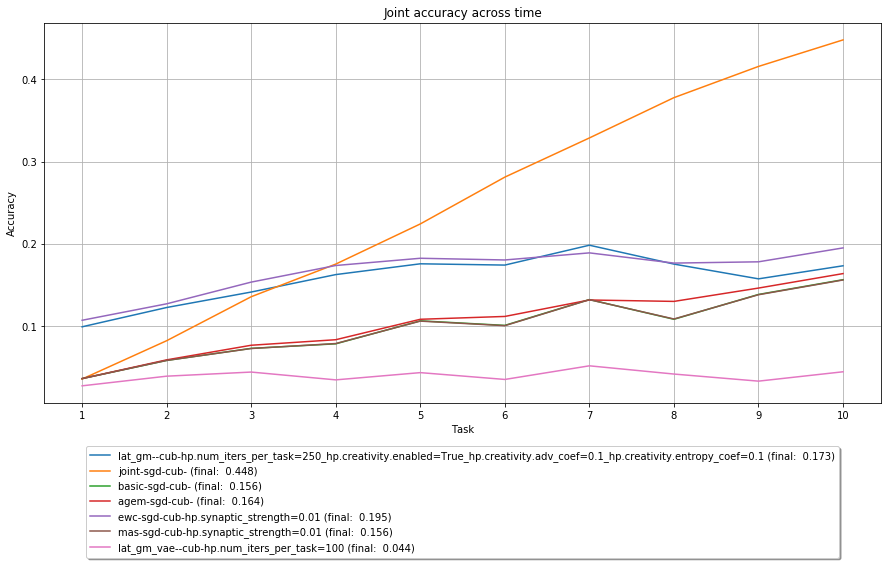
\includegraphics[width=0.8\textwidth]{images/early-scores.png}
        \caption{Joint accuracy on all the remaining unseen classes for CUB}
    \end{figure}
    
%    At first, we chose MeRGAN to apply the creativity loss to, but then ``realized'' that it will be more easy and fruitful to apply it in a feature space.
\end{frame}

\begin{frame}{What was done in November}

\begin{itemize}
    \item LGM-GAN on CUB dataset with the \textit{pretrained and fixed} embedder
    \item LGM-VAE on CUB dataset with the \textit{pretrained and fixed} embedder
    \begin{itemize}
        \item with/without the learned prior
        \item with/without class attributes in VAE/in Classifier
    \end{itemize}
    \item CL ``validation'' pipeline from A-GEM paper, trying different optimizers, trying model reinits, tweaking architectures, moving workflow into slurm, some metrics (LCA, forgetting speed) from A-GEM paper, fixing several bugs
\end{itemize}
\end{frame}

\begin{frame}{Why we have dropped MeRGAN}
    \pause
    \textbf{Fact}: original MeRGAN operates in the image space.
    
    \pause
    \textbf{Claim}: applying the creativity loss in the image space is not good.
    
    \pause
    \textbf{Justification}:
    \begin{itemize}
        \item In CIZSL, the creativity loss was applied to features, not images, i.e. we didn't have a good precedent of using the creativity loss in the image space to improve model's performance on unseen.
        \item It feels hard to manipulate images to generate sensible unseen images
        \item We would need a very big GAN model to do that, which is slower to train and harder to tune
    \end{itemize}
    
    \pause
    \textbf{Idea \#1}: let's apply creativity in the feature space, sticking closer to CIZSL
    
    \textbf{Problem}: where can we get these features?
    
    \pause
    \textbf{Idea \#2}: let's just use features from Classifier
\end{frame}

\begin{frame}{Using features from Classifier (1/3)}
    \pause
    \textbf{Claim} It doesn't work as is.
    
    \pause
    \textbf{Intuition}. Features drift away and LGM produces old features that are not only useless but even detrimental.
    
    \pause
    \textbf{Justification}
    \begin{figure}
        \centering
        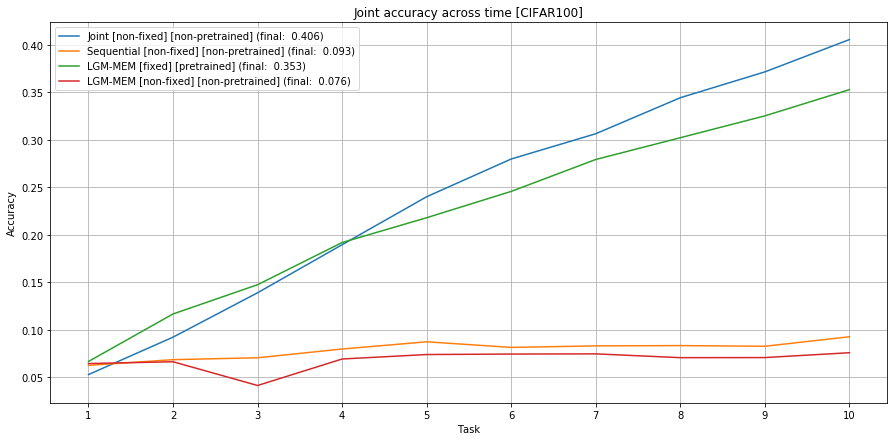
\includegraphics[width=0.8\textwidth]{images/lgm-mem-non-fixed-embedder-is-bad.png}
    \end{figure}
\end{frame}

\begin{frame}{Using features from Classifier (2/3)}
    \pause
    \textbf{Idea \#3}: what if we'll use a pretrained feature extractor?
    
    \pause
    \textbf{Claim}: it has 2 serious problems:
    \begin{itemize}
        \item\pause It \textit{feels} unfair to use pretrained models
        \item\pause It \textit{feels} not novel (ICCV19 paper does that, for example)
    \end{itemize}
    
    \pause
    \textbf{Idea \#4}: ok then, let's apply EWC to the Classifier to prevent features from drifting away.
    
    \pause
    \textbf{Claim}: it did not help, but I am sure I have a bug...
    
    \pause
    \textbf{Justification}
    \begin{figure}
        \centering
        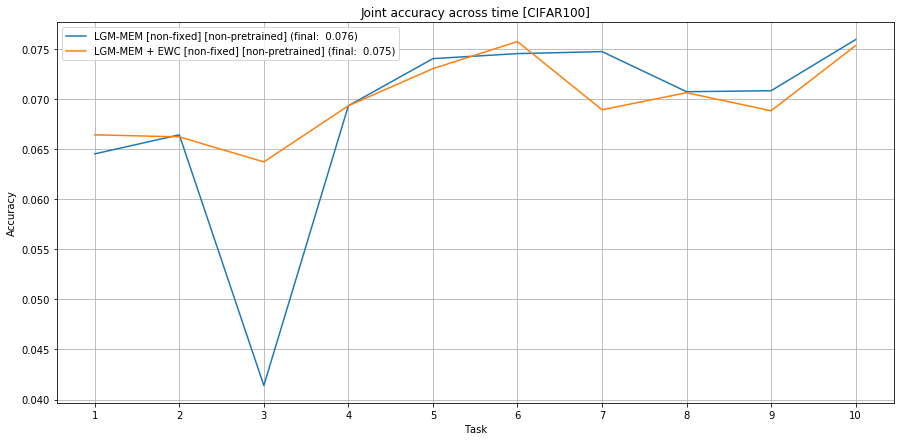
\includegraphics[width=0.8\textwidth]{images/lgm-mem-with-and-without-ewc.png}
    \end{figure}
\end{frame}

\begin{frame}{Using features from Classifier (3/3)}
    We can go into improving this approach, but let's step back for a while and think about LGM on top of the Classifier's features more generally. It has two serious problems:
    \begin{itemize}
        \item\pause We can't learn classes one by one like MerGAN can:
        \begin{itemize}
            \item\pause because of that it will not be a replacement for MeRGAN
            \item\pause because of that it will not be possible to use it in modern CL setups without task identity or task bounds
        \end{itemize}
        \item\pause Its performance will depend a lot on EWC performance
    \end{itemize}
\end{frame}

\begin{frame}{What was done in December}
    \begin{itemize}
        \item\pause Some small features: label smoothing, tuning joint baseline, etc
        \item\pause Add EWC/MAS regularization to LGM
        \item\pause Some bug fixes (proper GP calculation, metrics, model cloning, etc)
        \item\pause December was quite chaotic because of the conference, paperwork, holidays, etc...
    \end{itemize}
    
    \pause
    \begin{figure}
    \begin{subfigure}{.45\textwidth}
        \centering
        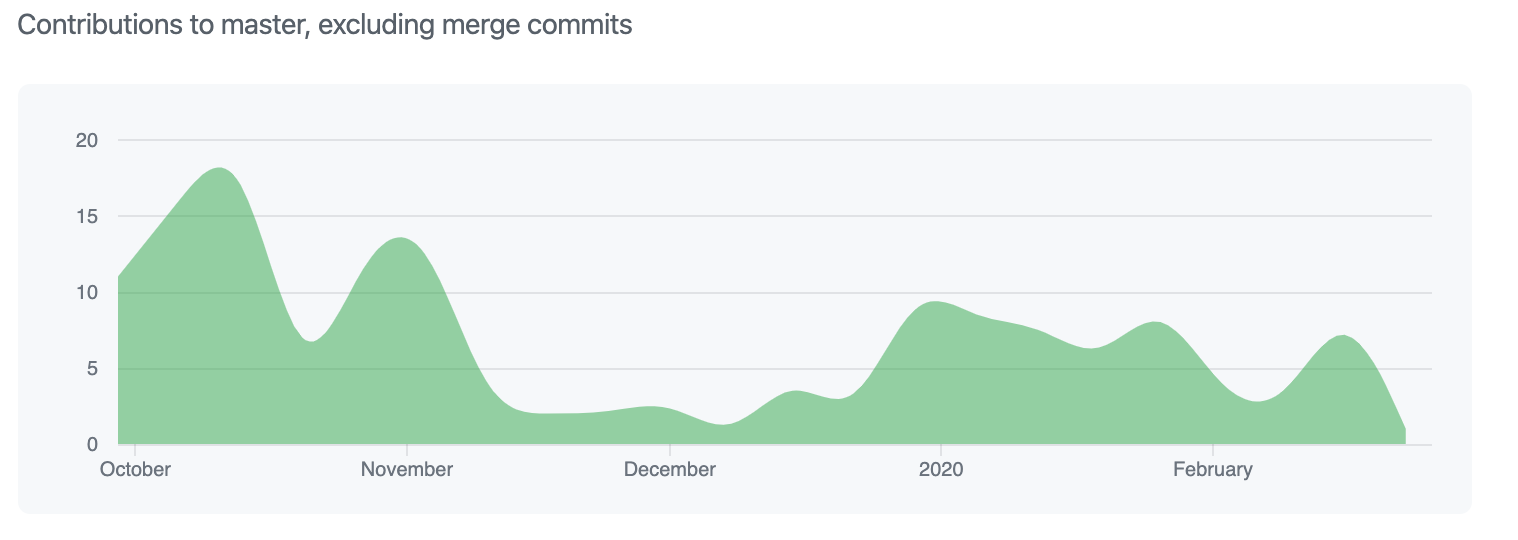
\includegraphics[width=\textwidth]{images/commits.png}
    \end{subfigure}
    \begin{subfigure}{.45\textwidth}
        \centering
        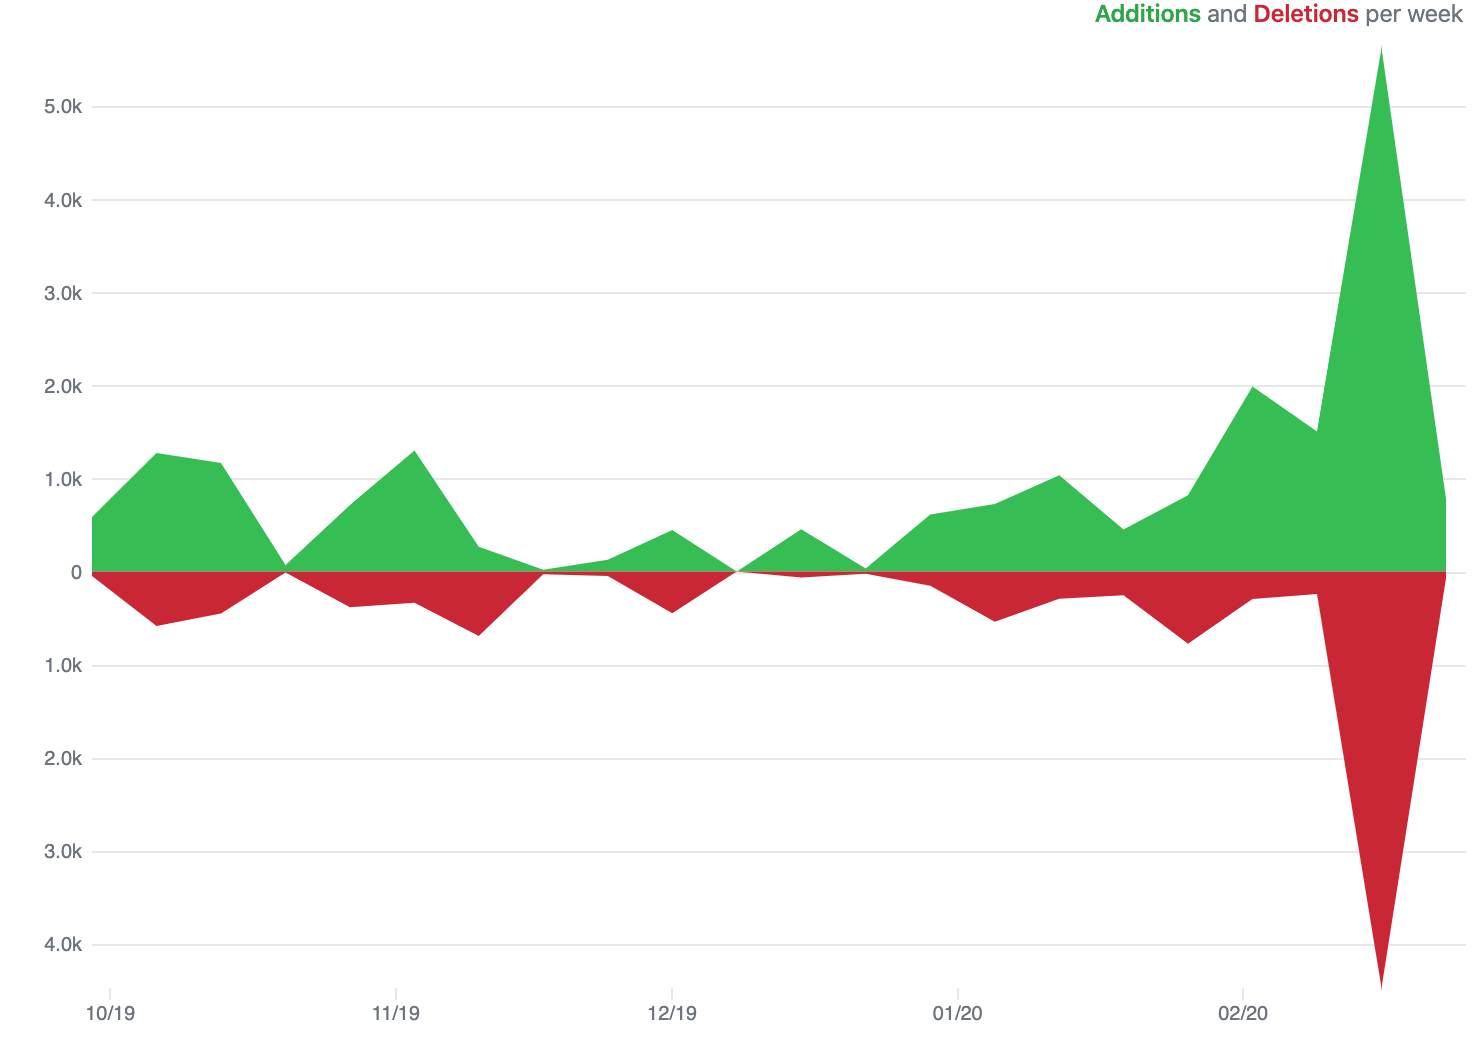
\includegraphics[width=\textwidth]{images/code-changes.png}
    \end{subfigure}
    \end{figure}
\end{frame}


\begin{frame}{What was done in January}
    \begin{itemize}
        \item\pause LGM-AC-GAN and LGM-VAE without attributes on CUB
        \begin{itemize}
            \item Result: 19.1\% and 33\% FJA.
        \end{itemize}
        \item\pause Convolutional LGM-GAN (like in ICCV19 paper) on CUB
        \begin{itemize}
            \item Result: performance dropped to 17.4\% FJA
        \end{itemize}
        \item\pause Creativity loss via simple entropy
        \begin{itemize}
            \item Result: nothing changed (but I didn't experiment a lot)
        \end{itemize}
        \item\pause Slow MeRGAN baseline on SVHN and AwA
        \begin{itemize}
            \item Result: 60\% CAS for SVHN
        \end{itemize}
        \item\pause Some small things: CL setup from ICCV19 paper (i.e. a large first task and small subsequent tasks), task transfer metric, etc.
        \begin{itemize}
            \item\pause Result: 37\% final joint accuracy on CUB (ICCV19 paper has 53\%, but they do a lot of ``cheating'')
        \end{itemize}
    \end{itemize}
\end{frame}

\begin{frame}{LGM-GAN vs LGM-VAE}
    \begin{figure}
        \centering
        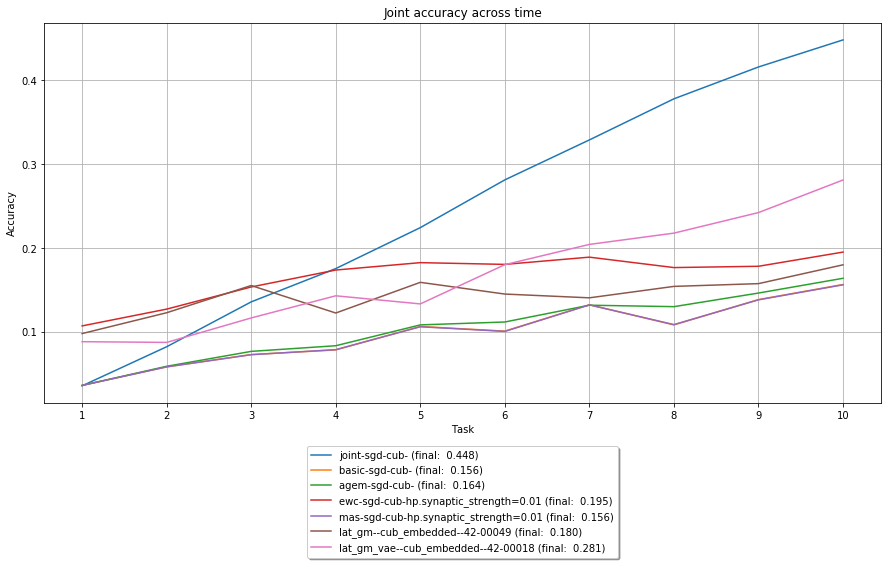
\includegraphics[width=\textwidth]{images/lgm-gan_vs_lgm-vae.png}
    \end{figure}
\end{frame}

{
%\usebackgroundtemplate{
%\begin{figure}
%    \begin{subfigure}{0.28\textwidth}
%        \centering
%        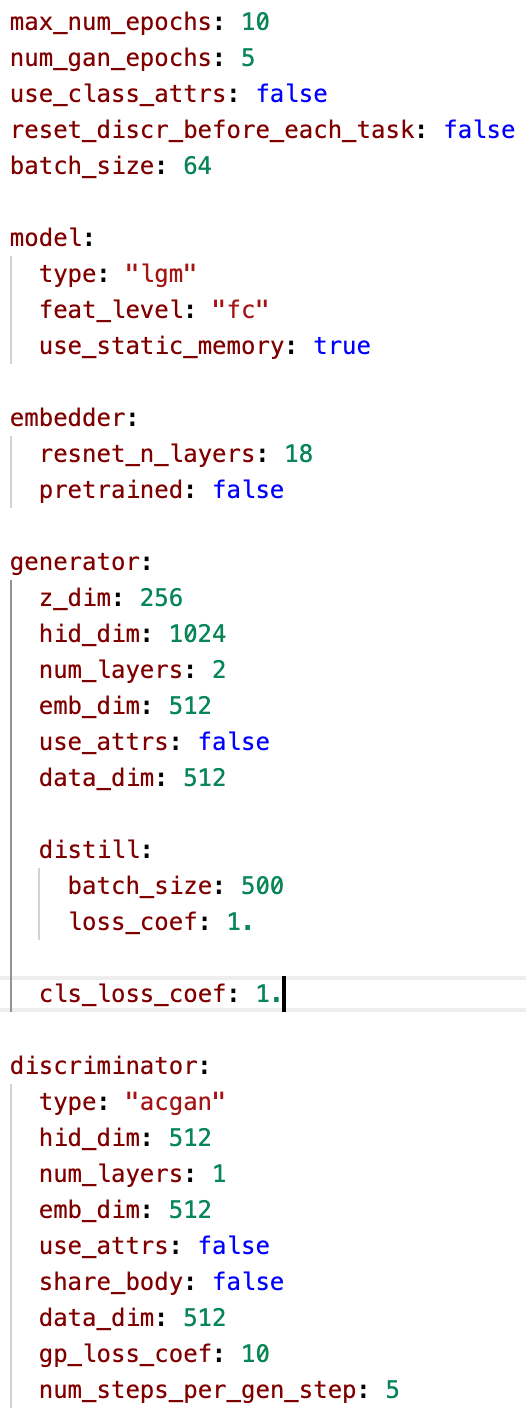
\includegraphics[width=\textwidth]{images/hps-screen-1.png}
%    \end{subfigure}
%    \begin{subfigure}{0.6\textwidth}
%        \centering
%        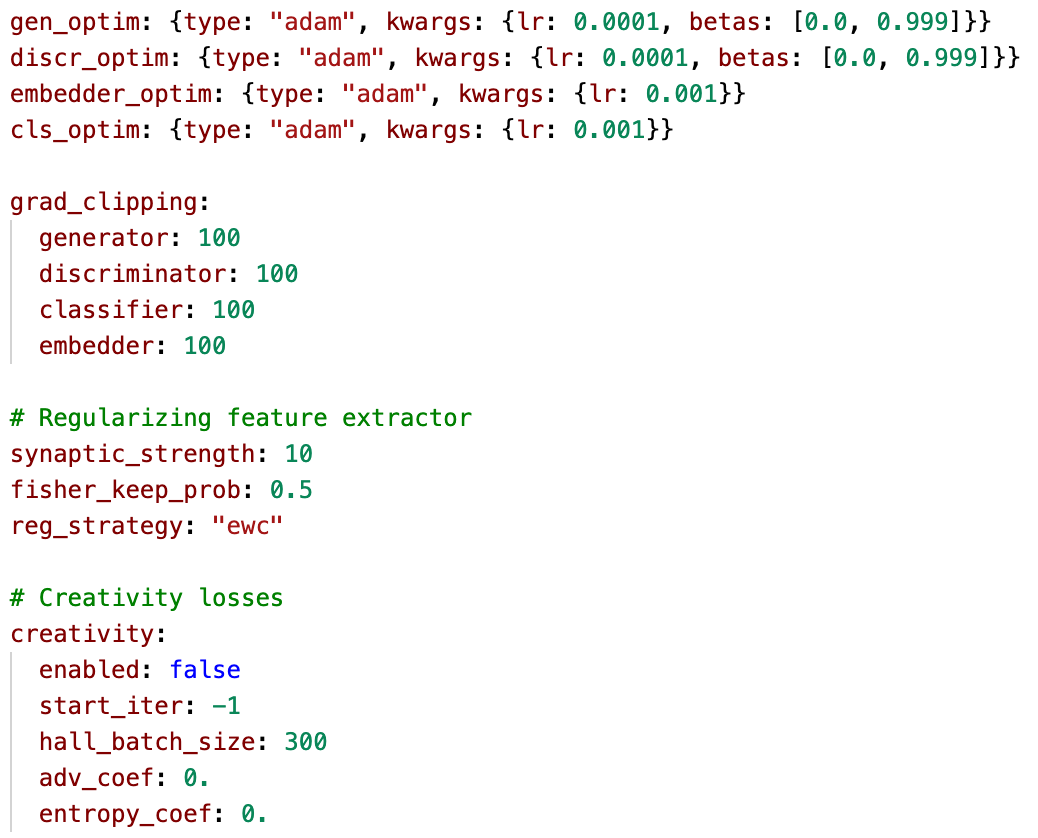
\includegraphics[width=\textwidth]{images/hps-screen-2.png}
%    \end{subfigure}
%\end{figure}
%}
%\usebackgroundtemplate{
%\centering
%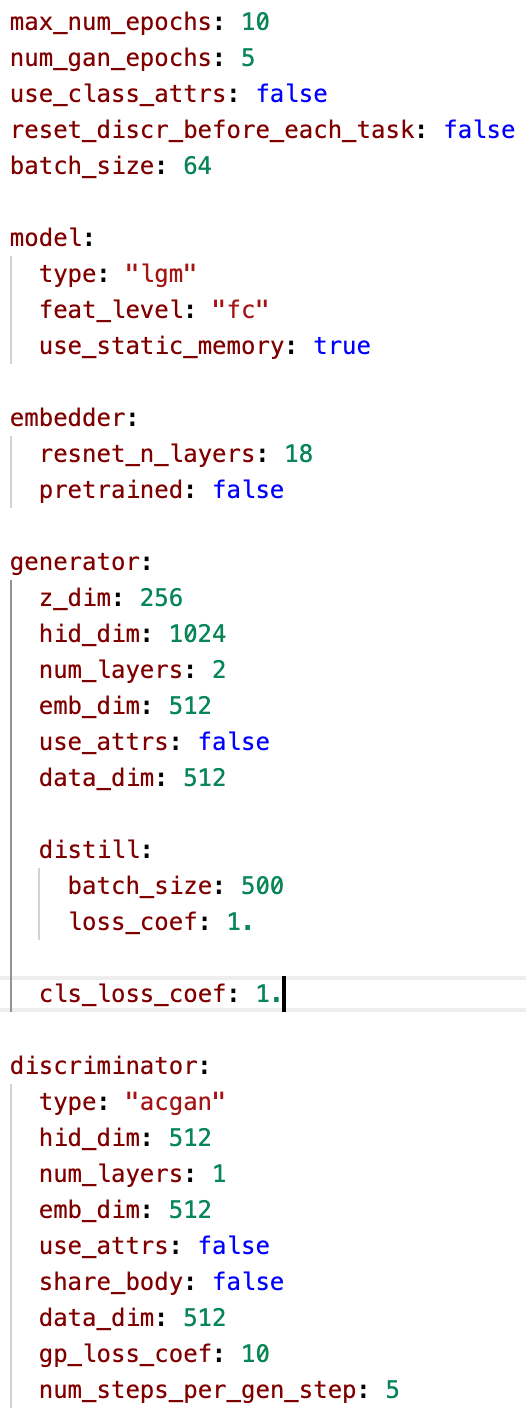
\includegraphics[width=0.3\textwidth]{images/hps-screen-1.png}
%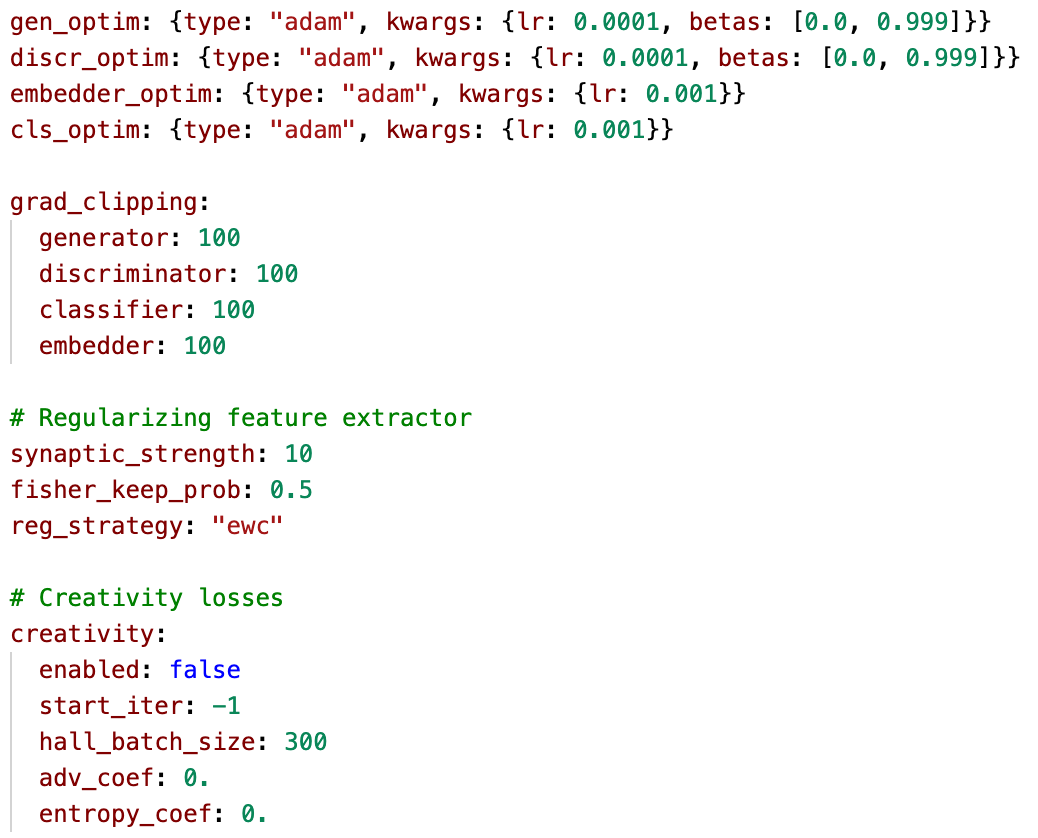
\includegraphics[width=0.3\textwidth]{images/hps-screen-2.png}
%}
\begin{frame}{LGM is cumbersome}
\begin{itemize}
    \item\pause Several terms (8 in total) in the objective:
    \begin{itemize}
        \item\pause AC-GAN losses: generator loss, generator classification loss, discriminator loss, classifier loss, gradient penalty
        \item\pause Generator prototypipcal loss
        \item\pause Rehearsal losses: generator rehearsal loss, classifier rehearsal loss
    \end{itemize}
    
    \item\pause Complex training scenario
    \begin{itemize}
        \item Continual learning involves several stages
        \item LGM/Classifier training stages
    \end{itemize}
    
    \item A lot of hyperparameters to tune:
    \begin{itemize}
        \item\pause Optimizers for each component
        \item\pause Resetting the components (Discriminator and Classifier)
        \item\pause AC-GAN vs cGAN
        \item\pause On which classes should we rehearse (seen or learned)
        \item\pause For how many epochs/steps
        \item\pause Architecture
        \item\pause etc
    \end{itemize}
\end{itemize}
\end{frame}
}

\begin{frame}{LGM via AutoEncoder}
    \textbf{Idea \#5} Let's extract features for LGM from autoencoder.
    \textbf{Details of training:}
    \begin{itemize}
        \item\pause Train an AutoEncoder sequentially on each task
        \item\pause For each task, train LGM on the features from AE
        \item\pause For each task, train Classifier on the features from AE
        \item\pause For each task, rehearse previous data from LGM to LGM
        \item\pause For each task, rehearse previous data from LGM to Classifier
        \item\pause For each task, rehearse previous data from LGM to AutoEncoder
    \end{itemize}
    
    \pause
    \textbf{Claim}: AE features are useless for classification
    
    \pause
    \textbf{Justification 1}: Joint classification score was only 29\% for CIFAR100 in my experiments
    
    \pause
    \textbf{Justification 2}: Joint classification score was only 31\% for CIFAR100 in Deep InfoMax paper (but their latent code size was smaller (64 dim), which improves classification).
\end{frame}

\begin{frame}{LGM via AutoEncoder (continued)}
    \pause
    \textbf{Claim}: since Classifier cannot learn to classify features, there is no reason to try LGM to learn to generate these class-conditional features.
    \textbf{Justification (hand-wavy)}: classification is an easier task than generation, so if we can't even classify the objects, there is not hope to learn to generate class-conditional objects.
    
    \pause
    \textbf{Idea \#6} (didn't try): we need to add classification objective into AutoEncoder's objective
    
    \pause
    \textbf{Problem}: but in this way we won't be able to learn classes one by one since our classification task will be singular (i.e. 1-class classification).
    
    \pause
    \textbf{Idea}: we can use already learned classes from LGM to fix that
    
    \pause
    \textbf{Potential problem}: AutoEncoder's performance can deteriorate because of this additional classification objective.
    
    \pause{Problem}: This will make the whole approach very cumbersome
\end{frame}


\begin{frame}{What was done in February}
    \begin{itemize}
        \item\pause Convolutional LGM-VAE on CUB
        \begin{itemize}
            \item\pause Result: 33\% FJA
        \end{itemize}
        \item\pause Since things didn't work, I started to decompose them and debug each component individually:
        \begin{itemize}
            \item\pause Training LGM-VAE, LGM-AC-GAN and LGM-cGAN independently to measure CAS on CUB and MNIST in a joint training scenario
            \begin{itemize}
                \item\pause Result: got 25\%, 22\% and 27\% CAS on CUB, 80\% vs 93\% CAS for LGM-AC-GAN and LGM-cGAN on MNIST (the goal was to get 98\%).
            \end{itemize}
            \item\pause Toy experiments on ``Memorizing Networks''
                \begin{itemize}
                    \item\pause Result: 0 MSE loss for memorizing 10k vectors of size 32 into LSTM.
                \end{itemize}
            \item\pause Training AutoEncoder on CIFAR10/CIFAR100 to incroporate later into LGM
            \begin{itemize}
                \item\pause Result: described on the previous slide.
            \end{itemize}
            \item\pause Training AutoEncoder continually to check its LLL properties
            \begin{itemize}
                \item Result: it does not forget previous data (it is interesting)
            \end{itemize}
        \end{itemize}
    \end{itemize}
\end{frame}

\begin{frame}{AutoEncoder does not forget previous data}
    \begin{figure}
        \centering
        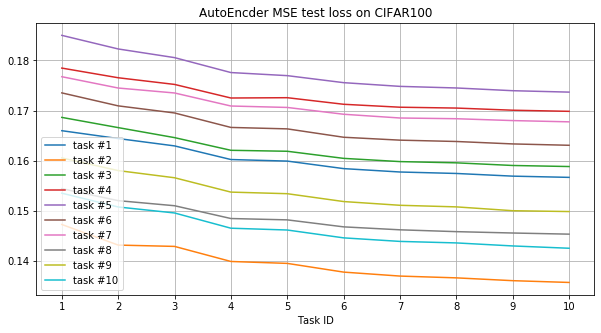
\includegraphics[width=\textwidth]{images/autoencoder-lll}
        \caption{MSE loss on different tasks for AutoEncoder trained sequentially}
    \end{figure}
\end{frame}

\begin{frame}{About ICCV19 paper}
    Honestly, there were problems in the paper and how the authors behaved:
    \begin{itemize}
        \item\pause Their approach is cumbersome
        \item\pause They are not clear about some important details
        \item\pause They try to conceal their research (do not provide the code, do not respond to emails)
    \end{itemize} 
    
    That's why I was unconsciously looking for reasons to drop their baseline:
    \begin{itemize}
        \item I think the way the authors do the research is not the way research should be done
        \item That's why I didn't want to build upon their work (why should we build upon it and spread it if the authors are hiding it?)
    \end{itemize}
\end{frame}

\begin{frame}{Conclusion}
    To build a good LGM one needs to solve 2 big problems:
    \begin{itemize}
        \item How to build a good feature extractor, i.e. a feature extractor that provides good features for a classifier.
        \item How to make its features not to drift away
    \end{itemize}
    
    \textit{And currently I do not have any concrete ideas to any of these problems.}
    
    \vspace{1em}
    
    Some thoughts:
    \begin{itemize}
        \item I do not want to drop the project because it feels like throwing away a 5-month work.
        \item But I do not see a concrete and principled idea of how to build LGM.
        \item Current LGM is already too cumbersome and I believe that cumbersome ideas do not survive unless they have outstanding results (like Mask R-CNN)
        %\item If we want to apply creativity loss in the image space then our baseline should be joint GAN training with evaluation on unseen, not MeRGAN.
    \end{itemize}
\end{frame}


\end{document}
